\documentclass[11pt]{article}

\usepackage[margin=1in]{geometry}
\usepackage[T1]{fontenc}
\usepackage[utf8]{inputenc}
\usepackage{lmodern}
\usepackage{amsmath}
\usepackage{amssymb}
\usepackage{booktabs}
\usepackage{array}
\usepackage{longtable}
\usepackage{enumitem}
\usepackage{graphicx}
\usepackage{float}
\usepackage{tikz}
\usepackage{hyperref}
\usepackage{xcolor}

\usetikzlibrary{arrows.meta, positioning}

\hypersetup{
  colorlinks=true,
  linkcolor=blue,
  urlcolor=blue,
  citecolor=blue
}

\title{CalWidget v2 Calibration Technical Documentation}
\author{EOVSAPY}
\date{\today}

\begin{document}
\maketitle

\tableofcontents

\section{Purpose and Scope}

This note documents the calibration logic implemented in the browser-native
CalWidget v2 path inside \texttt{eovsapy.calwidget\_html}. The goal is to give
an operator- and developer-facing description of what the code solves, what
state it stores, how interactive edits affect the solution, and what products
are exported to SQL or NPZ.

The document covers:
\begin{itemize}[leftmargin=1.5em]
  \item fine-channel reference calibration analysis for refcals,
  \item in-band delay fitting,
  \item relative phase modeling and residual diagnostics,
  \item time masking and band masking,
  \item manual and automatic flagging layers,
  \item exported sidecar and daily NPZ products,
  \item the intended operational workflow for HI and LO feed calibration.
\end{itemize}

This note does not attempt to replace the scientific notebooks. It describes the
current production-oriented implementation in the v2 widget.

\section{High-Level Calibration Model}

The v2 path treats a selected refcal as the anchor dataset for a given feed and
solves the calibration in layers:
\begin{enumerate}[leftmargin=1.5em]
  \item read and pre-correct fine-channel visibilities,
  \item fit one \emph{uniform in-band delay} per antenna and polarization,
  \item apply that delay to all fine channels,
  \item build a \emph{relative phase model} referenced to Antenna~1,
  \item diagnose remaining per-band residual phase and per-band residual delay,
  \item optionally apply a \emph{residual in-band correction},
  \item export the tuned model and flags.
\end{enumerate}

The design intentionally separates these layers because they solve different
problems:
\begin{itemize}[leftmargin=1.5em]
  \item the in-band delay solves the channel-scale phase slope within each band,
  \item the relative phase model solves the multi-band phase trend relative to
  the reference antenna,
  \item the residual diagnostics solve what remains after the previous two
  corrections and are used as a suggest-only or apply-on-click refinement path.
\end{itemize}

\begin{figure}[H]
  \centering
  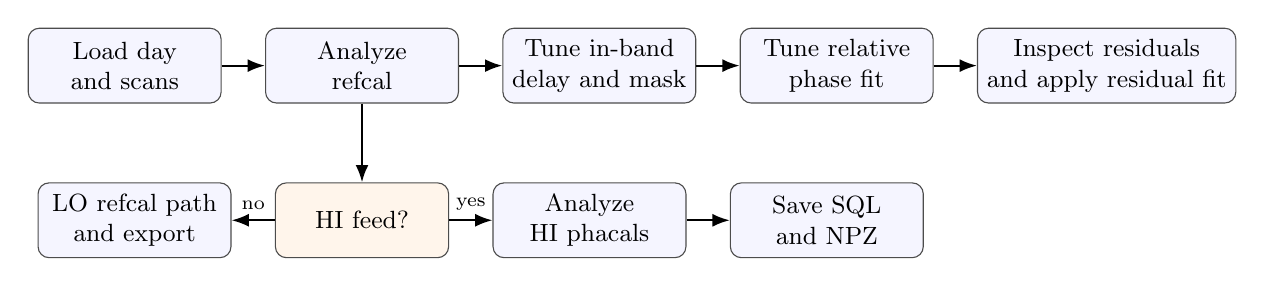
\begin{tikzpicture}[
    node distance=0.75cm and 0.55cm,
    block/.style={
      rectangle,
      rounded corners,
      draw=black!70,
      fill=blue!4,
      align=center,
      minimum width=2.45cm,
      minimum height=0.95cm,
      font=\small
    },
    decision/.style={
      rectangle,
      rounded corners,
      draw=black!70,
      fill=orange!8,
      align=center,
      minimum width=2.2cm,
      minimum height=0.95cm,
      font=\small
    },
    line/.style={-{Latex[length=2.2mm]}, thick}
  ]
    \node[block] (load) {Load day\\and scans};
    \node[block, right=of load] (refcal) {Analyze\\refcal};
    \node[block, right=of refcal] (inband) {Tune in-band\\delay and mask};
    \node[block, right=of inband] (relative) {Tune relative\\phase fit};
    \node[block, right=of relative] (residual) {Inspect residuals\\and apply residual fit};

    \node[decision, below=1.0cm of refcal] (feed) {HI feed?};
    \node[block, right=of feed] (phacal) {Analyze\\HI phacals};
    \node[block, right=of phacal] (export) {Save SQL\\and NPZ};
    \node[block, left=of feed] (lo) {LO refcal path\\and export};

    \draw[line] (load) -- (refcal);
    \draw[line] (refcal) -- (inband);
    \draw[line] (inband) -- (relative);
    \draw[line] (relative) -- (residual);
    \draw[line] (refcal) -- (feed);
    \draw[line] (feed) -- node[above, font=\scriptsize] {yes} (phacal);
    \draw[line] (phacal) -- (export);
    \draw[line] (feed) -- node[above, font=\scriptsize] {no} (lo);
  \end{tikzpicture}
  \caption{Operator workflow block diagram for CalWidget v2. The HI path includes
  in-band, relative-phase, and residual refinement before phacal analysis. The
  LO path remains separate.}
  \label{fig:workflow-block}
\end{figure}

\section{Inputs and Internal Data Products}

\subsection{Supported Inputs}

The refcal/phacal preparation path can ingest either:
\begin{itemize}[leftmargin=1.5em]
  \item raw IDB/UDB visibility data, or
  \item an NPZ file written by the legacy notebook/analysis path.
\end{itemize}

The imported scan is converted into a \texttt{ScanAnalysis} object that stores:
\begin{itemize}[leftmargin=1.5em]
  \item time stamps,
  \item source and scan metadata,
  \item layout information,
  \item fine-channel visibility cubes,
  \item corrected fine-channel visibility cubes,
  \item band-averaged products,
  \item time masks and flag products,
  \item the active delay solution and derived model state.
\end{itemize}

\subsection{Reference Frames and Symbols}

Throughout this note:
\begin{itemize}[leftmargin=1.5em]
  \item $a$ is the antenna index,
  \item $p \in \{X,Y\}$ is polarization,
  \item $b$ is the band index,
  \item $f$ is frequency in GHz unless stated otherwise,
  \item $\tau_{a,p}$ is a delay in ns,
  \item $\phi$ is wrapped phase in radians.
\end{itemize}

\section{Pre-Correction of Fine-Channel Visibilities}

\subsection{Feed Rotation and Parallactic-Angle Handling}

The v2 fine-channel path follows the same date-dependent behavior as the legacy
Tk widget:
\begin{itemize}[leftmargin=1.5em]
  \item before 2025-07-15, full X/Y feed-rotation and parallactic-angle
  unrotation are applied,
  \item from 2025-08-08 onward, only the Ant~4 parallactic-angle wrap fix is
  applied,
  \item between these dates the code follows the same cutoff logic as the
  legacy path.
\end{itemize}

This is important because applying the old full feed-rotation correction to
later data changes the fine-channel phase pattern and breaks consistency with
legacy calibration products.

\subsection{Time-Drift Correction}

Before fitting in-band delays, the code applies a legacy-style time-drift
correction in the fine-channel domain. For each antenna and polarization:
\begin{enumerate}[leftmargin=1.5em]
  \item a per-band time slope is fit from the band-averaged phase versus time,
  \item only bands with phase-fit scatter below a quality cutoff are kept,
  \item a median drift coefficient is formed,
  \item all fine channels in a band are rotated by the corresponding time drift.
\end{enumerate}

This makes the fine-channel fitting path more consistent with the legacy band
workflow and reduces slow time-dependent phase drift before delay solving.

\section{Uniform In-Band Delay Solution}

\subsection{Per-Band Linear Phase Fit}

For each antenna $a$, polarization $p$, and fitted band $b$, the code computes a
linear phase fit
\begin{equation}
  \phi_{a,p,b}(f) \approx \phi_{0,a,p,b} + 2\pi f \tau_{a,p,b}.
\end{equation}

The per-band solve stores:
\begin{itemize}[leftmargin=1.5em]
  \item \texttt{per\_band\_delay\_ns},
  \item \texttt{per\_band\_phase0},
  \item \texttt{per\_band\_std}.
\end{itemize}

\subsection{Notebook-Matched Weighted Mean}

The fitted uniform in-band delay is the weighted mean over valid per-band
delays:
\begin{equation}
  \tau^{\mathrm{fit}}_{a,p}
  =
  \frac{\sum_b w_{a,p,b}\tau_{a,p,b}}
       {\sum_b w_{a,p,b}},
  \qquad
  w_{a,p,b} = \frac{1}{\sigma_{a,p,b}^2}.
\end{equation}

The important implementation choice is that $\sigma_{a,p,b}$ is kept as the raw
phase-fit scatter returned by \texttt{lin\_phase\_fit}, in radians. It is
\emph{not} converted into a delay-domain uncertainty. This matches the notebook
reference path and avoids over-weighting wider high-frequency bands.

\subsection{Applied Delay Convention}

The active delay is applied to all channels in a band using the band midpoint:
\begin{equation}
  V'_{a,p}(f)
  =
  V_{a,p}(f)\,
  \exp\left[
    -i\,2\pi \tau^{\mathrm{active}}_{a,p}
    \left(f - f_{\mathrm{mid},b}\right)
  \right].
\end{equation}

This removes the fitted in-band slope without forcing an arbitrary phase shift
at the band center.

\section{Delay-Solution State}

The active refcal stores the in-band and relative-fit state in a
\texttt{DelaySolution} object. The main fields are:
\begin{itemize}[leftmargin=1.5em]
  \item \texttt{fitted\_ns}: notebook-matched fitted in-band delay,
  \item \texttt{active\_ns}: currently applied in-band delay,
  \item \texttt{relative\_ns}: display-only multiband relative correction,
  \item \texttt{kept\_band\_mask}: main in-band mask for the in-band delay solve,
  \item \texttt{residual\_kept\_band\_mask}: residual-panel-specific mask,
  \item \texttt{residual\_auto\_band\_mask}: residual auto mask,
  \item \texttt{manual\_ant\_flag\_override}: operator whole-antenna flag layer,
  \item \texttt{manual\_ant\_keep\_override}: operator whole-antenna keep layer.
\end{itemize}

The main kept-band mask and the residual kept-band mask are intentionally
separate. The former controls the main in-band delay solution. The latter
controls only the residual in-band refinement path.

\section{Relative Phase Model}

\subsection{Reference Convention}

The relative phase panel uses Antenna~1 as the reference.
\begin{itemize}[leftmargin=1.5em]
  \item For Antenna~1, the panel displays the corrected absolute phase.
  \item For antennas $a>1$, the panel displays the corrected phase of
  Antenna~$a$ relative to Antenna~1.
\end{itemize}

\subsection{Joint X/Y Constraint}

The model uses both X and Y polarization together. The code assumes that
$Y-X$ is approximately constant for a given antenna after delay correction, so
the X and Y phase tracks are not fit independently. The procedure is:
\begin{enumerate}[leftmargin=1.5em]
  \item compute delay-corrected X and Y phases,
  \item estimate a circular mean $Y-X$ offset,
  \item align the X and Y tracks to one shared phase branch,
  \item fit a shared phase model,
  \item reconstruct the Y model by re-applying the fitted $Y-X$ offset.
\end{enumerate}

\subsection{Antenna-Dependent Model Class}

The code uses different model classes for the reference and non-reference
antennas:
\begin{itemize}[leftmargin=1.5em]
  \item \textbf{Antenna~1}: a weighted Chebyshev polynomial model on the coarse
  band-sampled phase trend,
  \item \textbf{Antennas 2+}: a weighted linear model in frequency.
\end{itemize}

Low frequency is up-weighted by a factor proportional to $1/\sqrt{f}$ to reduce
the leverage of noisy high-frequency channels.

\subsection{Manual Relative Correction}

The \texttt{Relative Phase Delay Editor} applies a display-only additional delay
on top of the automatically fit multiband baseline. For non-reference antennas
the slope changes, then the intercept is re-fit from the time-averaged
fine-channel data so the line is anchored back to the data after the slope edit.

This path is separate from the in-band delay editor:
\begin{itemize}[leftmargin=1.5em]
  \item \textbf{Anchor Refcal Delay Editor}: changes the applied in-band delay
  \texttt{active\_ns},
  \item \textbf{Relative Phase Delay Editor}: changes the displayed multiband
  relative-fit overlay only.
\end{itemize}

\section{Residual Diagnostics}

\subsection{Per-Band Residual Phase}

After the relative model is formed, the code computes residual phase by
subtracting the model from the corrected phase and re-wrapping the difference to
$[-\pi,\pi]$.

The residual panel shows two different fit layers:
\begin{itemize}[leftmargin=1.5em]
  \item \textbf{Multiband Fit} in red: the residual-guided multiband suggestion
  path,
  \item \textbf{Inband Fit} in blue: an in-band style linear fit computed
  separately within each band from the residual phase.
\end{itemize}

\subsection{Residual Delay Per Band}

The residual delay panel computes, for each band, a post-correction scalar delay
estimate from the corrected complex visibility. It also computes an all-band
residual delay estimate. These are diagnostics; they are not the primary fit.

\subsection{Residual-Specific Masking}

The residual panel now has its own mask state, independent of the main in-band
kept-band mask. The purpose is to exclude obviously bad bands from the residual
in-band refinement without altering the main in-band fit window.

The residual auto mask uses two gates:
\begin{enumerate}[leftmargin=1.5em]
  \item residual phase scatter gate:
  \begin{equation}
    \sigma^{\mathrm{res}}_{a,p,b} \le \sigma_{\mathrm{thr}},
  \end{equation}
  where $\sigma_{\mathrm{thr}}$ is a user-adjustable residual scatter threshold,
  defaulting to 1.0 rad,
  \item residual delay robust outlier gate:
  \begin{equation}
    \left|\tau^{\mathrm{res}}_{a,p,b} - \mathrm{median}(\tau^{\mathrm{res}})\right|
    \le 3\,\mathrm{MAD}(\tau^{\mathrm{res}}).
  \end{equation}
\end{enumerate}

If too few bands are finite or the MAD is zero, the delay gate is disabled and
only the scatter gate is used.

\subsection{Apply Residual Fit}

When the operator clicks \texttt{Apply Residual Fit}, the code:
\begin{enumerate}[leftmargin=1.5em]
  \item commits any staged residual masks,
  \item computes one residual in-band correction per antenna and polarization
  from the committed residual mask,
  \item adds that correction to \texttt{active\_ns} for all antennas and both
  polarizations,
  \item rebuilds corrected diagnostics and dependent products.
\end{enumerate}

This path does \emph{not} change:
\begin{itemize}[leftmargin=1.5em]
  \item the main kept-band mask used by the original in-band solve,
  \item the multiband relative baseline fit state.
\end{itemize}

\section{Automatic and Manual Antenna Flagging}

\subsection{Y-X Residual RMS}

For each antenna, the code computes a $Y-X$ residual RMS from the difference
between the observed $Y-X$ phase and the fitted constant $Y-X$ model. This is a
quality metric for phase consistency between the two polarizations.

The threshold is operator-adjustable in the \texttt{Relative Phase + Fit}
section. The current default is 1.5 rad.

\subsection{Flag Layers}

Three layers of flag semantics are kept distinct:
\begin{itemize}[leftmargin=1.5em]
  \item \texttt{legacy\_flag}: legacy/SQL-style flag array,
  \item \texttt{v2\_flag}: current tuned v2 flag state,
  \item \texttt{model\_flag}: export flag state for the fitted model path.
\end{itemize}

In the interactive relative-phase panel, whole-antenna manual keep/flag
overrides are stored separately from the automatic threshold decision. This
allows the operator to bring back an automatically flagged antenna or exclude a
nominally acceptable one.

\section{Time Masking}

Time masking is handled in the browser-native time-history path. The main ideas
are:
\begin{itemize}[leftmargin=1.5em]
  \item intervals are defined in Julian Date,
  \item multiple antenna-band targets can share one interval group,
  \item staged time masks are queued until the operator clicks
  \texttt{Apply Mask},
  \item the heatmap distinguishes pending and committed masked cells.
\end{itemize}

The fine-channel diagnostic plots use time-averaged visibilities after applying
the active browser time-mask state. Therefore a time-mask update changes the
data shown in the in-band and residual panels.

\section{Scan Classification and Feed Separation}

HI and LO feed scans are handled separately. The code attempts to classify feed
kind from scan metadata such as project and FSeq information, with duration used
only as a fallback when explicit metadata is unavailable.

Operationally:
\begin{itemize}[leftmargin=1.5em]
  \item HI and LO refcals should be solved separately,
  \item HI phacals use the tuned HI reference model,
  \item LO calibration usually does not require the same relative multiband
  phase refinement depth as HI.
\end{itemize}

\section{Persistence}

\subsection{Refcal Sidecar}

Each tuned refcal can write a sidecar NPZ under
\texttt{/common/webplots/phasecal}. The sidecar stores the fitted and active
delay solution, mask state, manual flag overrides, and scan metadata. The
sidecar is used to restore the calibration state when returning to the same
refcal.

\subsection{Daily Model NPZ Export}

The daily bundle export writes one NPZ archive containing one entry per analyzed
scan. For each exported scan, the bundle stores:
\begin{itemize}[leftmargin=1.5em]
  \item fine-channel frequency grid,
  \item band frequency grid,
  \item fitted model phase on the fine grid,
  \item fitted model phase on the band grid,
  \item \texttt{legacy\_flag},
  \item \texttt{v2\_flag},
  \item \texttt{model\_flag},
  \item manual antenna keep/flag overrides,
  \item $Y-X$ residual RMS and threshold,
  \item scan metadata.
\end{itemize}

Flags are saved as explicit arrays. The phase arrays are \emph{not} encoded by
blanking or NaN-masking to indicate flags.

\section{Frontend Payload Architecture}

The browser uses three top-level data channels:
\begin{itemize}[leftmargin=1.5em]
  \item heatmap payload,
  \item time-history payload,
  \item overview payload.
\end{itemize}

Within the overview payload, each plot section has its own payload builder. The
server can return:
\begin{itemize}[leftmargin=1.5em]
  \item a full overview object, or
  \item \texttt{overview\_updates} containing only the sections affected by a
  given action.
\end{itemize}

This split is important for performance:
\begin{itemize}[leftmargin=1.5em]
  \item initial load fetches all top-level payloads,
  \item many button actions return only the relevant patched sections,
  \item sparse per-antenna edits can update only one antenna's panels.
\end{itemize}

\begin{figure}[H]
  \centering
  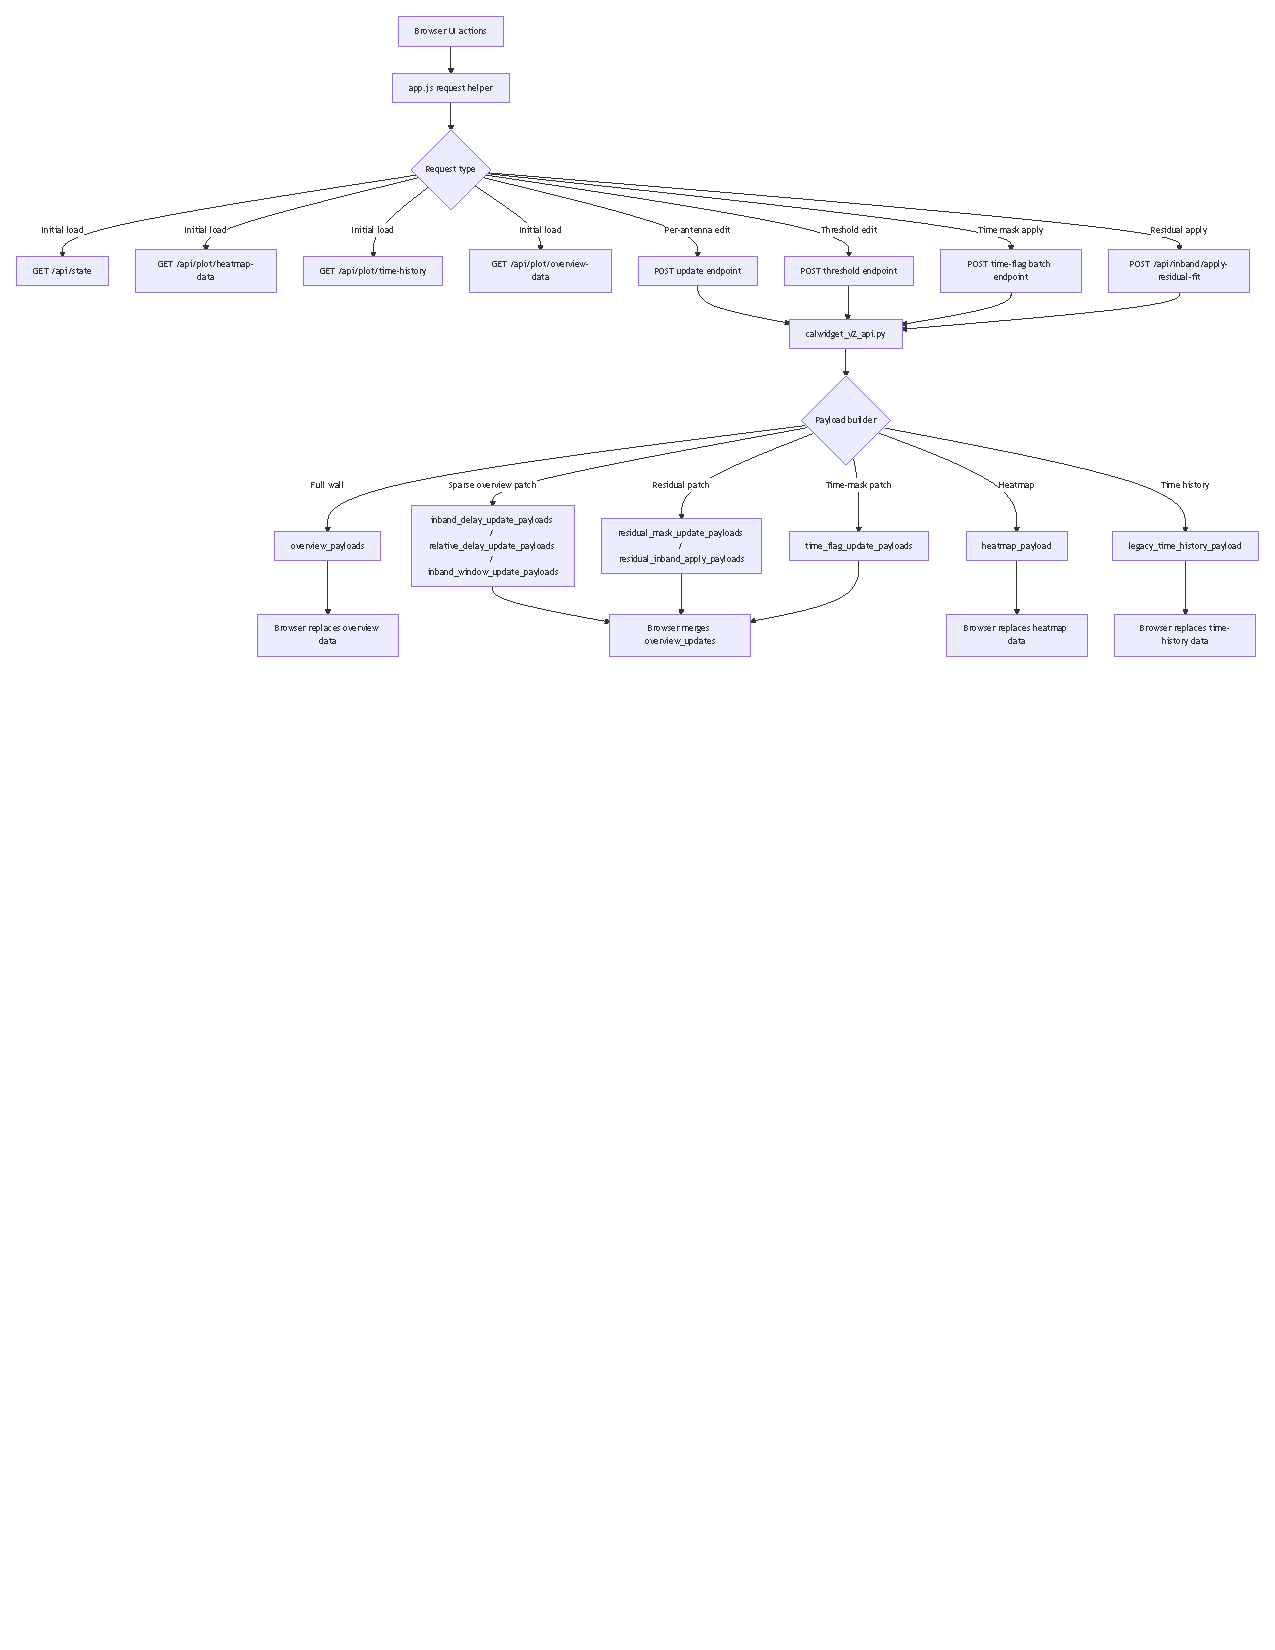
\includegraphics[width=\textwidth]{diagrams/calwidget_v2_api_flow.pdf}
  \caption{API payload flow. Initial page load uses separate top-level fetches,
  while most interactive actions return scoped payload patches.}
  \label{fig:api-flow}
\end{figure}

\begin{figure}[H]
  \centering
  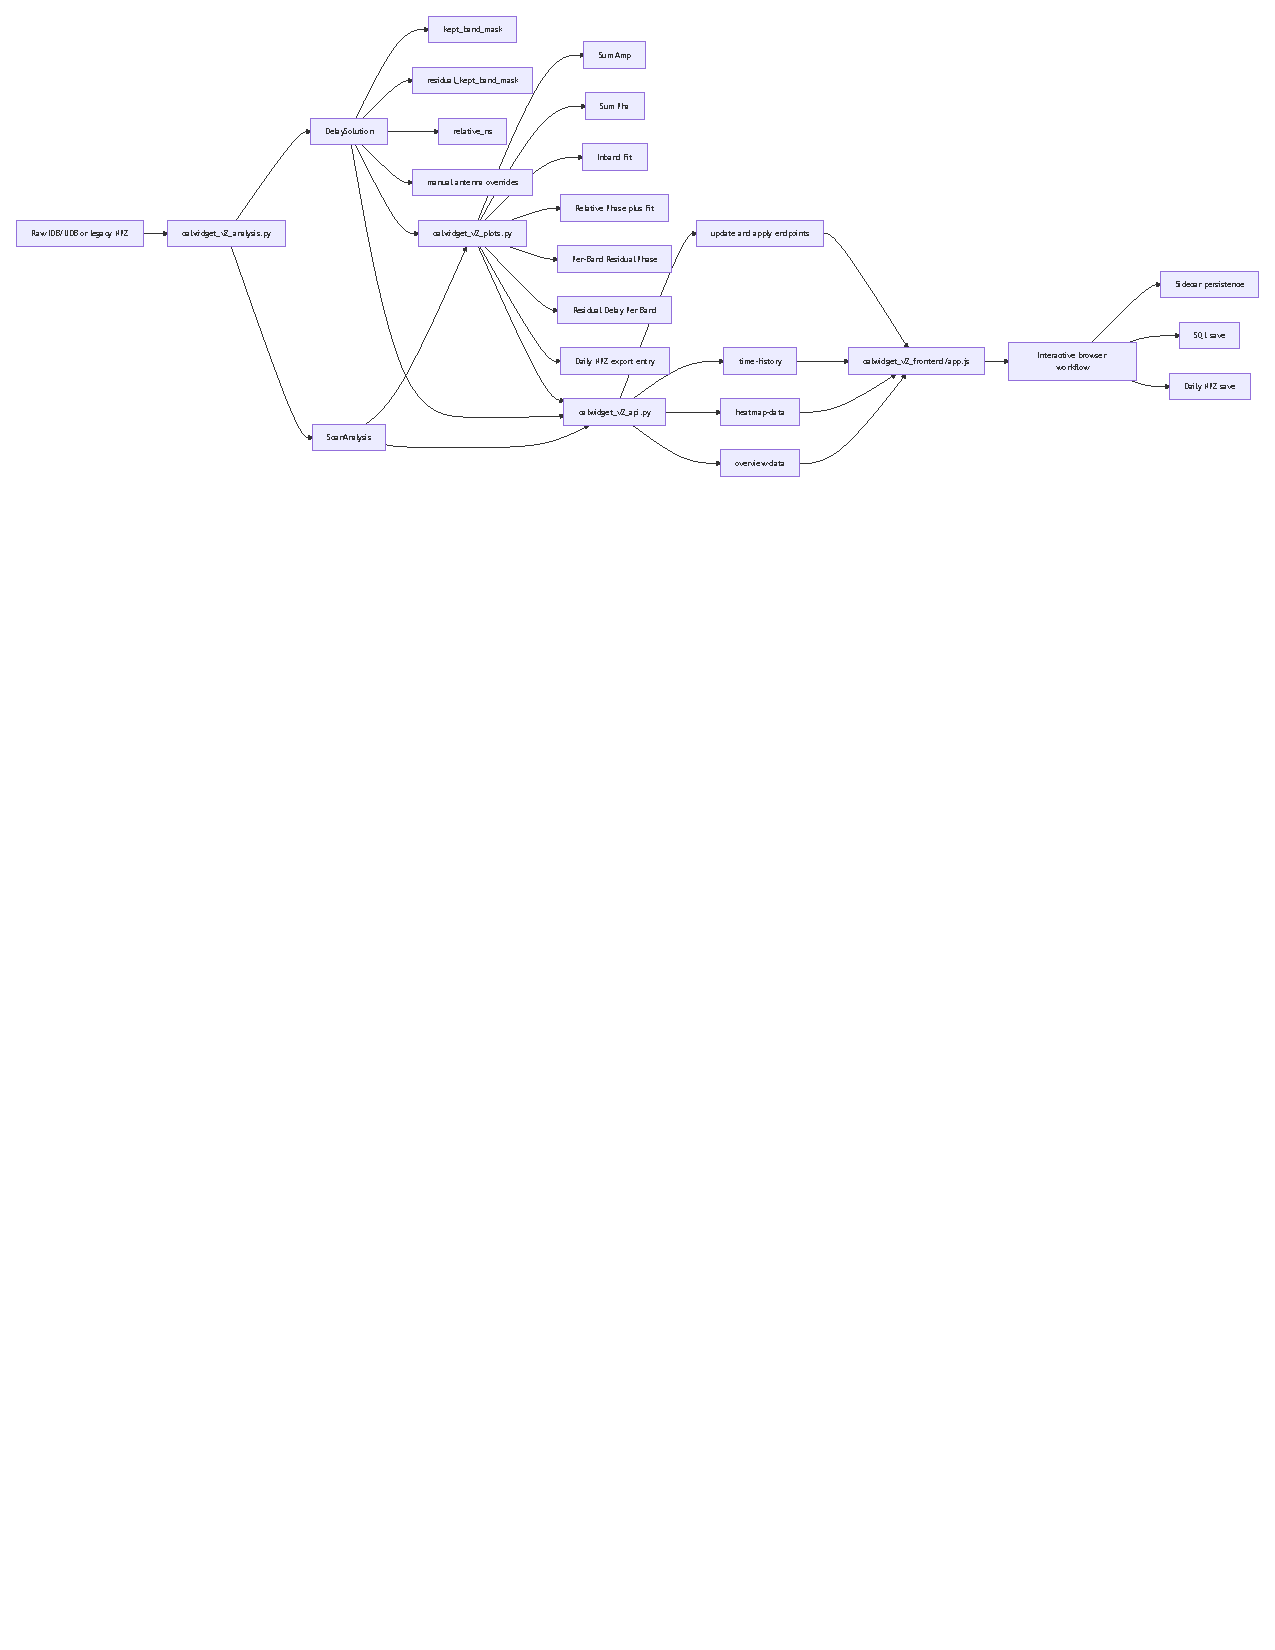
\includegraphics[width=\textwidth]{diagrams/calwidget_v2_code_architecture.pdf}
  \caption{Code architecture for the v2 calibration path. Analysis state,
  payload generation, API routing, frontend interaction, and export are
  separated into distinct modules.}
  \label{fig:code-architecture}
\end{figure}

\section{Recommended Operator Workflow}

\subsection{High Feed}

The intended HI workflow is:
\begin{enumerate}[leftmargin=1.5em]
  \item select and analyze one HI refcal,
  \item tune the in-band delay mask and solve,
  \item inspect \texttt{Relative Phase + Fit},
  \item apply multiband relative suggestions only when needed,
  \item inspect \texttt{Per-Band Residual Phase},
  \item tune residual masks and apply residual fit,
  \item verify flags, $Y-X$ residual RMS, and whole-antenna keep/flag decisions,
  \item analyze the HI phacals,
  \item save SQL products as needed,
  \item save the daily NPZ bundle.
\end{enumerate}

If both morning and evening HI refcals exist, the operator may:
\begin{itemize}[leftmargin=1.5em]
  \item use only one anchor, or
  \item choose one canonical anchor and keep the second as secondary drift
  metadata.
\end{itemize}

\subsection{Low Feed}

The LO workflow is separate:
\begin{enumerate}[leftmargin=1.5em]
  \item analyze the LO refcal,
  \item verify amplitude and phase consistency,
  \item save LO products,
  \item export to the daily NPZ bundle if desired.
\end{enumerate}

\section{Known Boundaries}

The current implementation has several explicit boundaries:
\begin{itemize}[leftmargin=1.5em]
  \item the multiband and residual correction paths are separate by design,
  \item residual masking affects residual in-band refinement only,
  \item the Chebyshev Antenna~1 model is an analytic approximation, not a full
  physical instrument model,
  \item the daily NPZ export writes whatever products already exist in the
  current session; it does not synthesize missing analyses.
\end{itemize}

\section{File Map}

The main implementation files are:
\begin{itemize}[leftmargin=1.5em]
  \item \texttt{eovsapy/calwidget\_html/calwidget\_v2\_analysis.py} for scan
  preparation, delay-solution state, masking state, and sidecar persistence,
  \item \texttt{eovsapy/calwidget\_html/calwidget\_v2\_plots.py} for diagnostic
  model generation and export payloads,
  \item \texttt{eovsapy/calwidget\_html/calwidget\_v2\_api.py} for the HTTP API,
  \item \texttt{eovsapy/calwidget\_html/calwidget\_v2\_frontend/app.js} for the
  browser interaction model.
\end{itemize}

\section{Summary}

CalWidget v2 is not just a re-skin of the legacy widget. It is a layered
fine-channel calibration system with explicit state for:
\begin{itemize}[leftmargin=1.5em]
  \item notebook-matched in-band delay fitting,
  \item joint X/Y multiband relative phase modeling,
  \item residual-specific bad-band masking,
  \item manual and automatic antenna flagging,
  \item sidecar persistence and daily model export.
\end{itemize}

That separation is the main design principle of the v2 path. It keeps the
operator in control while still allowing partial automation and reproducible
exports.

\end{document}
